Para analizar la efectividad y ecuanimidad de esta nueva forma de calcular el ranking vamos a realizar una serie de test a fin de obtener un analisis cuantitativo y cualitativo 
que nos permita compararlo con el clásico método de \textbf{WP}. \\
Con los test esperamos encontrar ventajas y desventajas de esta forma de medición, particularmente en escenarios donde no todos los participantes juegen la misma cantidad de partidos.
\\

Además realizaremos una comparación de los métodos de \textbf{Eliminación Gaussiana} y \textbf{Cholesky} para ver cual de los dos computa los rankings de manera mas eficiente.
\\

En esta sección solo presentaremos los experimentos realizados y los resultados obtenidos. Las conclusiones de cada experimento
las presentaremos en la seguiente sección. 


\subsection{Ranking}

Vamos a comparar la tabla de ranking obtenida a partir de un set de datos de la \textbf{ATP 2007}. Es decir calculamos el ranking a partir de la técnica \textbf{WP}, considerando 
partidos ganado \/ partidos jugados, a pesar de que no todos los jugadores hayan participado de la misma cantidad de partidos. Comparandolo con el \textbf{CMM} implementado con \textbf{Cholesky}. \\


\begin{figure}[H]
\centering
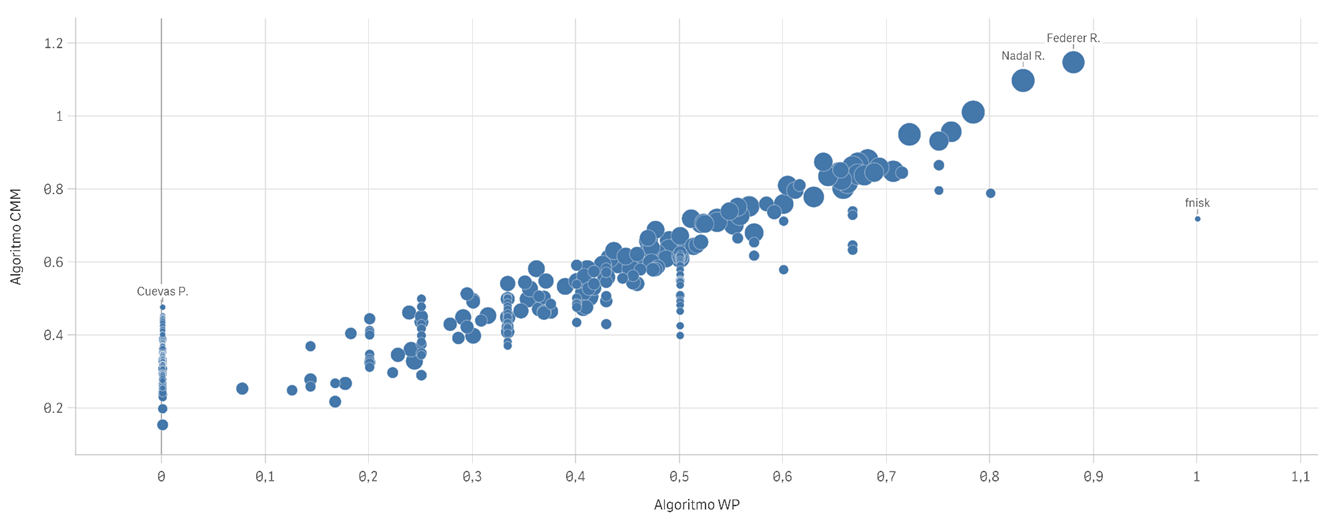
\includegraphics[width=1\textwidth]{IMG/Comparativa WP- CMM todos.png}
\caption{Rankings para comparar WP vs CMM}
\label{fig:Comparacion de tecnicas}
\end{figure}

\\
El grafico elegido para graficar es un grafico de dispersion, que muestra: \\

\begin{itemize}
	\item Eje X el valor obtenido al ejecutar el algoritmo WP.
	\item Eje Y el valor obtenido al ejecutar CMM implementado con Cholesky.
	\item El tamaño de la burbuja es la cantidad de partidos jugados.
\end{itemize}

	
Lo que se observa en el grafico es que el ranking CMM parece darle relevancia a la cantidad de partidos jugados ya que las burbujas de los top 10 son mas grandes.
Esto esta dado en principio por la caracteristica del deporte (tenis) que permite a los que ganan jugar mas partidos en los torneos. 
Lo que nos llamo la atencion es que si observamos el rank arrojado por WP, se observa que el primero es fnisk. El mismo es un jugador que solo jugo 1 partido y lo gano, 
por lo cual tiene un 100 \% de efectividad y figura como primero. \\
Ademas, si observamos los top 10 del rank WP, observamos algunas burbujas de tamaño pequeño. Esto es porque en algunos casos, este ranking beneficia jugar pocos 
partidos pero ganarlos.
\\

Hemos realizado un zoom dentro del grafico para corroborar el nombre y posicion de ambos rankings.
\\

\begin{figure}[H]
\centering
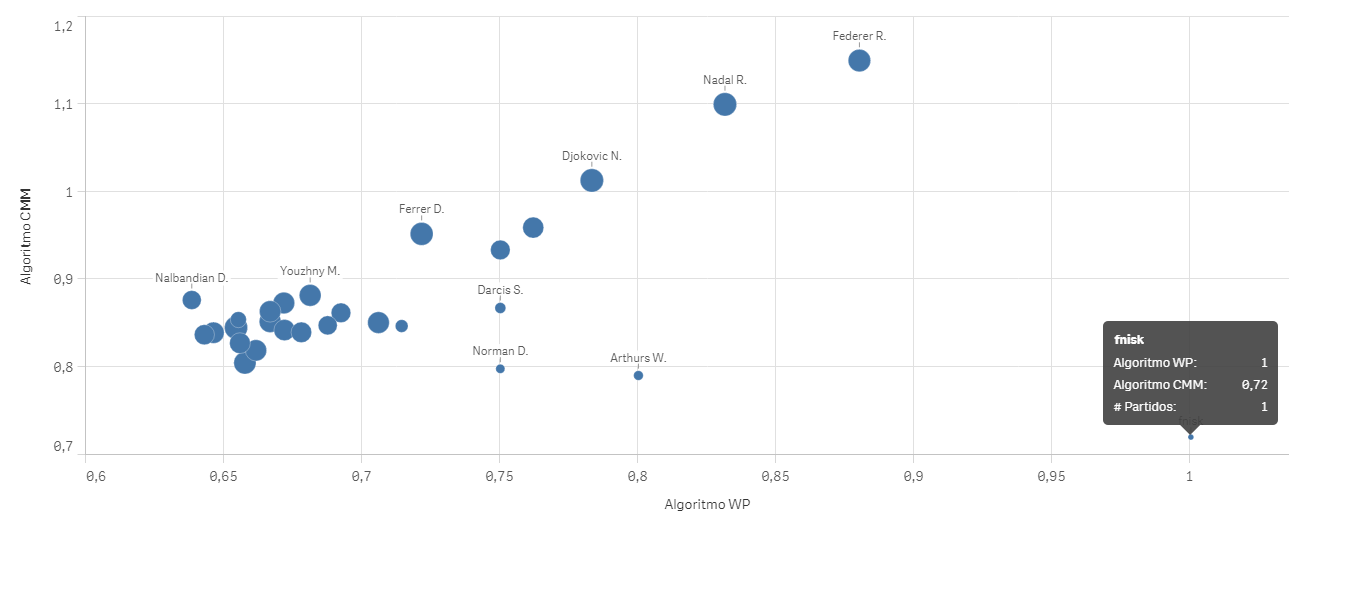
\includegraphics[width=1\textwidth]{IMG/comparativa WP - CMM zoom.png}
\caption{Zoom de las primeras posiciones}
\label{fig:Zoom de las primeras posiciones}
\end{figure}

\\ 
En el grafico se resalta el jugador fnisk y se muestra informacion adicional.
\\

\subsection{¿Importa a quien se le gana?}


En el escenario que se utilize \textbf{WP} realmente no importa a que equipo se le gane, ya que todos los partidos tienen la misma importancia y se les asigna el mismo puntaje. Pero en el caso de \textbf{CMM} resulta mas interesante plantearse esta pregunta. \\

La hipótesis que tenemos es que tomando un equipo de mitad de tabla, que denominamos \textbf{medio} el hecho de que le gane al lider de la tabla va a mejorar mucho mas el ranking que derrotando al que ocupe la última posición. \\

Realizamos un test tomando al equipo \textbf{medio}, y agregando un partido victorioso contra el puntero y analizamos como se modifica su ranking. Luego tomamos la tabla inicial, es decir sin ganarle al puntero, y repetimos el experimento esta vez derrotando al último. \\

Presentamos los resultados obtenidos.

\\

\begin{table}[ht]
\caption{Posicion Inicial}
\centering
\begin{tabular}{c c c}
\hline \hline
    Posición & Jugador & Ranking \\ 
    \hline

    1 & Federer & 1,131919 \\ 
    164 & Vasallo Arguello & 0,474265 \\ 
    334 & Vicente F. & 0,198425 \\ 
  
    \end{tabular}
\end{table}

\begin{table}[ht]
        \caption{Ganandole al Primero}

\centering
\begin{tabular}{c c c}
\hline \hline
    Posición & Jugador & Ranking \\ 
    \hline

    1 & Federer & 1,117437 \\ 
    141 & Vasallo Arguello & 0,508447 \\ 
    334 & Vicente F. & 0,198271 \\ 
    \hline
    \end{tabular}
\end{table}

\begin{table}[ht]
\caption{Ganandole al Ultimo}
\centering
\begin{tabular}{c c c}
\hline \hline
    Posición & Jugador & Ranking \\ 
    \hline
    1 & Federer & 1,132469 \\ 
    141 & Vasallo Arguello & 0,480302 \\ 
    334 & Vicente F. & 0,170821 \\ 
    \hline
    \end{tabular}
\end{table}

\newline


Se observa una mejoria en el ranking luego de haber ganado contra el primero.
\\



\subsection{Racha ganadora}

Para estudiar la ecuanimidad del \textbf{CMM} realizamos un experimento tomando al participante del \textbf{ATP 2007} que se encontraba en el último puesto y le asignamos una racha ganadora contra los primeros diez jugadores del ranking. \\

Además este test nos permite observar como la racha de un jugador afecta al ranking global y si ganandole a los mejores realmente escala una considerable cantidad de posiciones en el ranking. \\

A continuación presentamos el ranking calculado construido de la siguiente manera: \\

\begin{itemize}
	\item Eje X el valor obtenido al ejecutar CMM implementado con Cholesky.
	\item Eje Y el valor obtenido al ejecutar CMM implementado con Eliminación Gaussiana.
	\item El tamaño de la burbuja es la cantidad de partidos jugados.
\end{itemize}

\\

\begin{figure}[H]
\centering
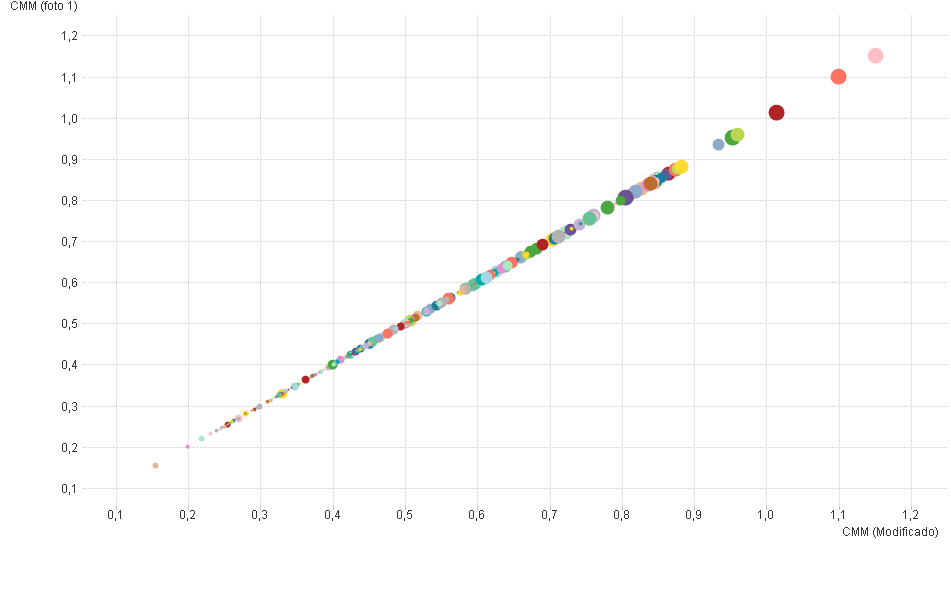
\includegraphics[width=1\textwidth]{IMG/comparativa cmm -cmm foto 0.png}
\caption{Ranking de jugadores}
\label{fig:Ranking de jugadores}
\end{figure}

\\
Es logico que se observe una diagonal ya que ambos ejes son la misma metrica de CMM.
\\
Luego el experimento realizado fue agregar partidos al schedule, de manera que el ultimo le gane a los 10 primeros y entender que tipo de reaccion tiene el algoritmo CMM.
\\
Para ello se realizaron 10 schedules distintos de tal forma que en cada uno de esos archivos de entrada exista un partido mas que en el caso anterior y
el mismo sea una victoria del ultimo jugador del ranking vs alguno de los top 10.

\\
Para poder mostrar una evolucion a medida que se van jugando los 10 partidos, hemos dejado el eje Y del grafico con el ranking inicial, mientras que el eje X paso a ser el ranking recalculado con la agregacion de partidos.\\
En el gráfico se observa mediante una flecha el salto del ranking de un partido a otro y evidencia cual es la ganancia que se tiene al ganarle a los top 10. 
\\

\begin{figure}[H]
\centering
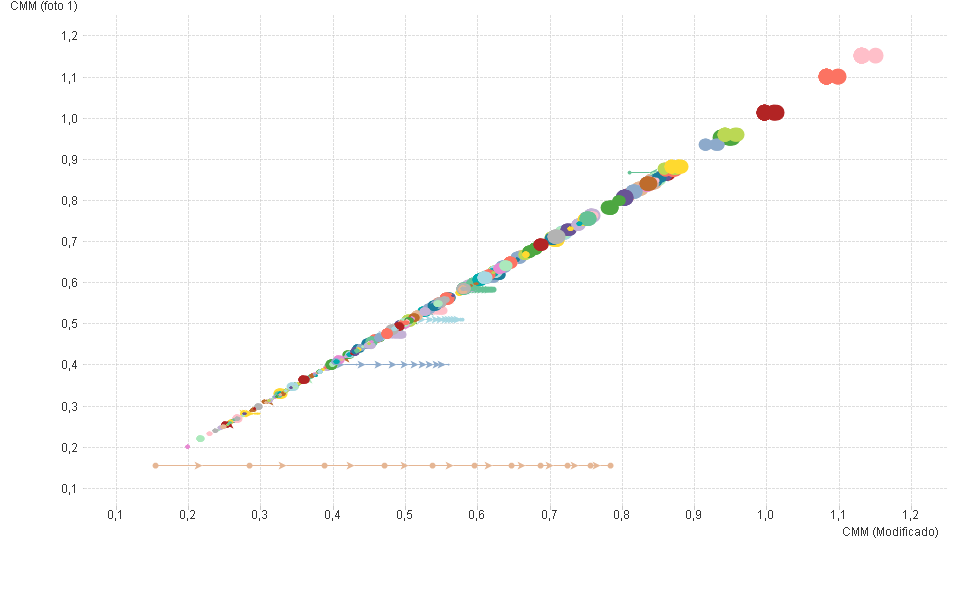
\includegraphics[width=1\textwidth]{IMG/comparativa cmm -cmm foto 10.png}
\caption{Evolucion de jugadores con el pasar de los partidos}
\label{fig:Evolucion de jugadores con el pasar de los partidos}
\end{figure}

\\
Por ultimo y para entender si el jugador en la ultima posicion podia llegar a ser primero en algun momento, hemos agregado al archivo un total de 100 partidos ganados por el ultimo contra 
los top 10.
\\

\begin{figure}[H]
\centering
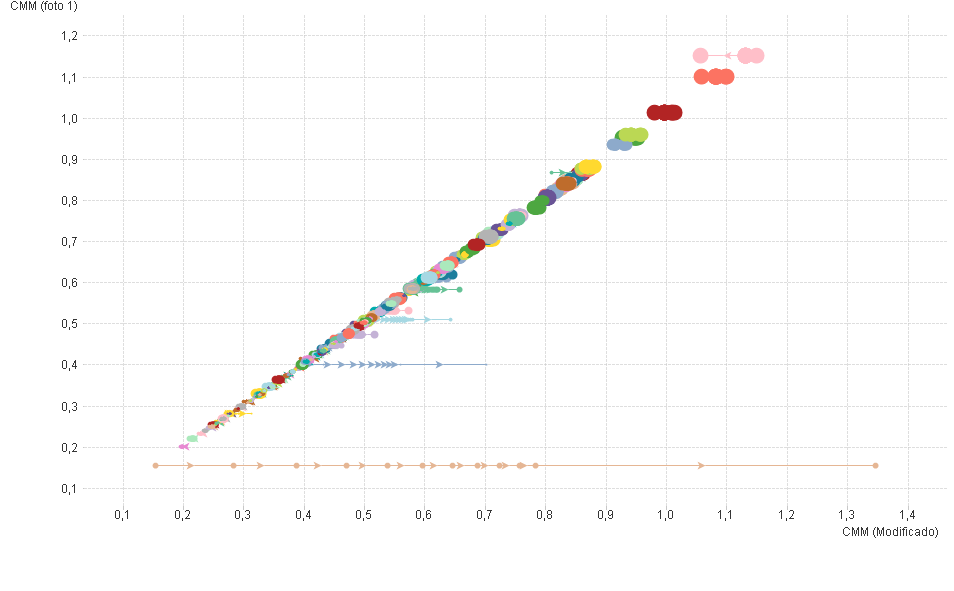
\includegraphics[width=1\textwidth]{IMG/comparativa cmm -cmm foto 100.png}
\caption{Evolucion de jugadores con el pasar de los partidos}
\label{fig:Evolucion de jugadores con el pasar de los partidos}
\end{figure}

\\
Y tal como vemos, si es posible pero a un costo altisimo (jugar alrededor de 100 partidos).
\\
Lo interesante es que aquellos equipos contra los que el ultimo jugador jugo tambien sufrieron modificaciones en su ranking. \\
A continuacion se observa un zoom dentro del grafico para observar este comportamiento.
\\

El ultimo jugador del ranking se llama Verkerk M., sus partidos fueron los siguientes:
\\
\begin{figure}[H]
\centering
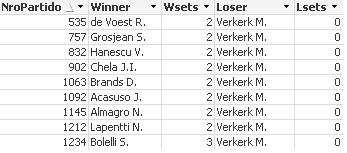
\includegraphics[width=1\textwidth]{IMG/partidos jugados vs verkerk.png}
\caption{Partidos jugados por Verkerk}
\label{fig:Partidos jugados por Verkerk}
\end{figure}

\\
En el siguiente grafico se observa el movimiento de ranking de los que le ganaron partidos a Verkerk, teniendo en cuenta la escalada al primer puesto de este jugador.
\\
\begin{figure}[H]
\centering
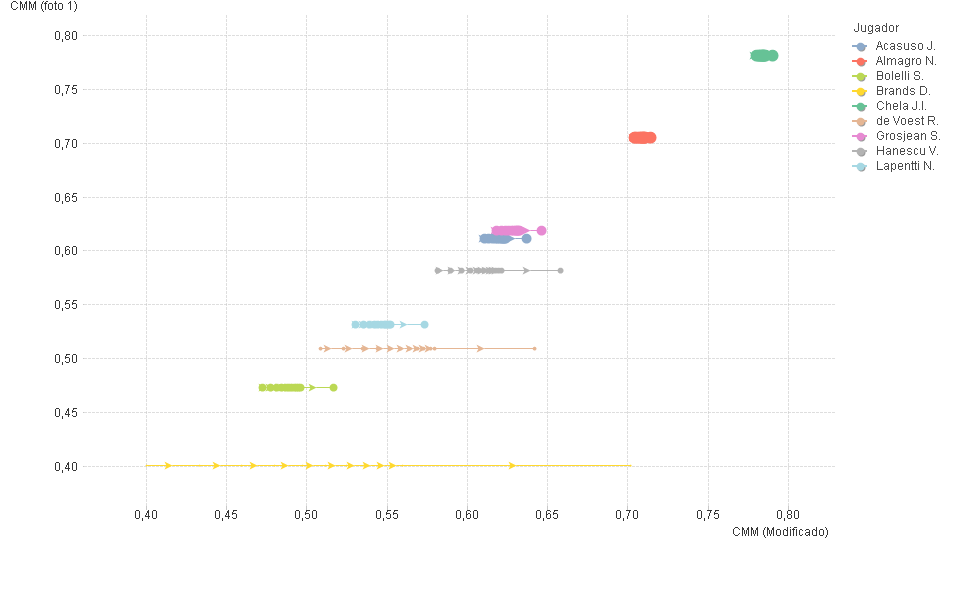
\includegraphics[width=1\textwidth]{IMG/partidos jugados vs verkerk grafico.png}
\caption{Evolucion de aquellos que le ganaron a Verkerk}
\label{fig:Evolucion de aquellos que le ganaron a Verkerk}
\end{figure}

\subsection{Escalando Posiciones}

Una de las consignas del trabajo era encontrar una tecnica para hacer escalar en el ranking a un \textbf{equipo}, pensamos en 2 tacticas. 
\\
Ambas se basan en, dado un schedule ya definido donde existe un jugador que esta ultimo en el ranking, hacerlo jugar y ganar vs 'el que siempre esta primero en la fecha correspondiente' y 'contra el que tiene inmediatamente arriba de el en el rank'
\\
Pensamos en una primera instancia era que tenia que ascender mas pronto aquel jugador que juega y gana contra el que ocupa el primer puesto que aquel que juega y gana contra cualquier otro jugador.
\\
Los algoritmos realizados cortan la ejecucion al llegar al primer puesto, arrojando la cantidad de partidos en total que debio jugar, y ganar, ese jugador.

A continuacion se muestran los graficos.


\subsubsection{Ganarle siempre al primero}

\begin{figure}[H]
\centering
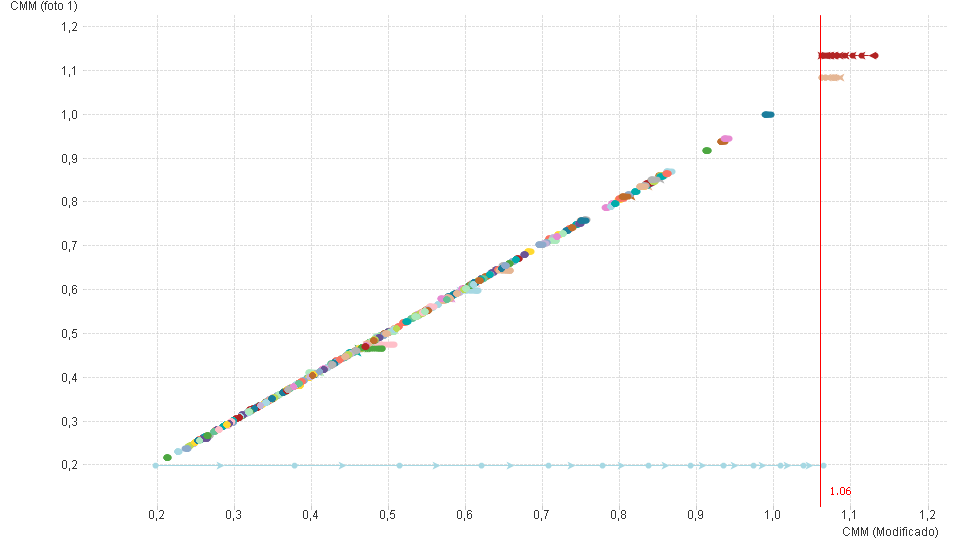
\includegraphics[width=1\textwidth]{IMG/estrategia 5.png}
\caption{Ganarle siempre al primero}
\label{fig:Ganarle siempre al primero}
\end{figure}

En este grafico se observa lo siguiente.\\
Cada burbuja es un jugador, el eje de las X es el rank que arroja CMM para las distintas fechas jugadas, mientras que el eje Y tiene el rank de CMM base para 
realizar el analisis y comparar la evolucion de los jugadores.

En este grafico se observa que el crecimiento es rapido en un incio y luego va reduciendo su velocidad de crecimiento.
Se observa que el algoritmo necesita de 12 fechas para llegar a la cima del campeonato, validando nuestra teoria.\\

Se observa tambien una linea de referencia que indica cuando llega el jugador a superar al primero del ranking.\\

\subsubsection{Ganarle al que esta inmediatamente arriba}
\\

\begin{figure}[H]
\centering
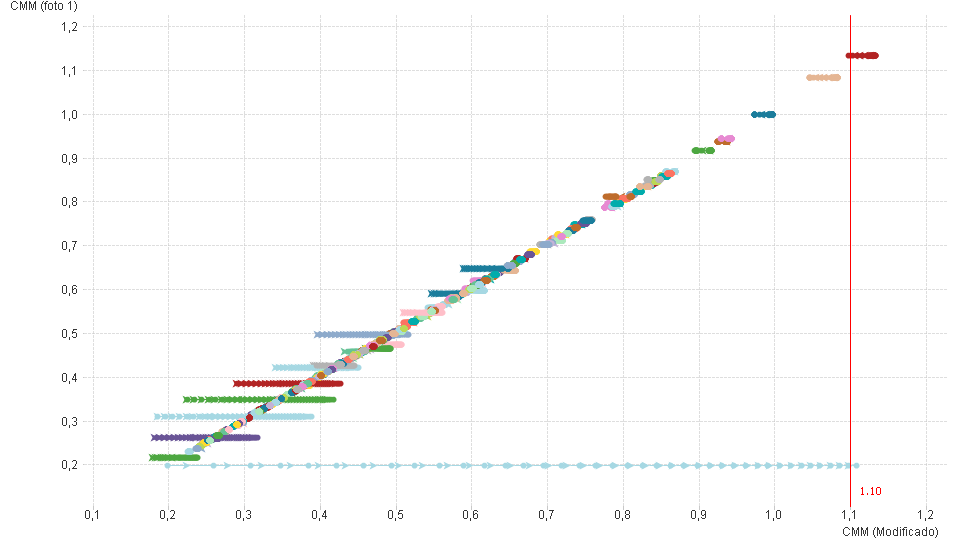
\includegraphics[width=1\textwidth]{IMG/estrategia 4.png}
\caption{Ganarle siempre al que esta inmediatamente arriba}
\label{fig:Ganarle siempre al que esta inmediatamente arriba}
\end{figure}

En este grafico se observa que el crecimiento es lento y que se necesitan aproximadamente 40 fechas para llegar a la cima del campeonato.\\

Se observa tambien una linea de referencia que indica cuando llega el jugador a superar al primero del ranking.\\


\subsection{Analisis Cuantitativo}


Vamos a estudiar la eficiencia de ambas tecnicas incrementando y variando los volúmenes de datos. La idea es repetir el cómputo de los rankings para la misma instancia de datos al azar, 
y posteriormente ir incrementando la cantidad de datos. \\

Nuestra hipótesis es el que método de basado en \textbf{WP} va a tardar lo mismo para instancias de datos iguales, y se irá incrementando de forma casi lineal a medida que 
incrementemos los datos. En cambio con \textbf{CMM} basando en \textbf{Eliminación Gaussiana} y \textbf{Cholesky} esperamos que difieran en para las mismas intancias. 
Nuestra hipótesis sobre esto es que la implementación de \textbf{Cholesky} va a demorar menos tiempo. \\

Para esta prueba se generaron schedules variando la cantidad de equipos en 6, 50, 100, 200, 300, 500, 700, 1000 y 2000. \\

Adicionalmente se varió la cantidad de partidos jugados por cada equipo. Dado el análisis de complejidad de los algoritmos implementados, solo varían el tiempo de calculo en 
funcion del tamaño de la matriz definida por la cantidad de equipos, por lo cual al variar la cantidad de partidos no esperamos encontrarnos con variaciones en el tiempo. \\

Ejecutamos los test para nuestra implementación de Eliminación Gaussiana.A continuación se muestran los resultados de tiempos de ejecucion dependiendo la cantidad de equipos.
Para evidenciar la complejidad cubica del algoritmo lo hemos encerrado entre 2 funciones cuadraticas que evidencian que no pueden contener la curva de tiempos de nuestro algoritmo. \\


\begin{figure}[H]
\centering
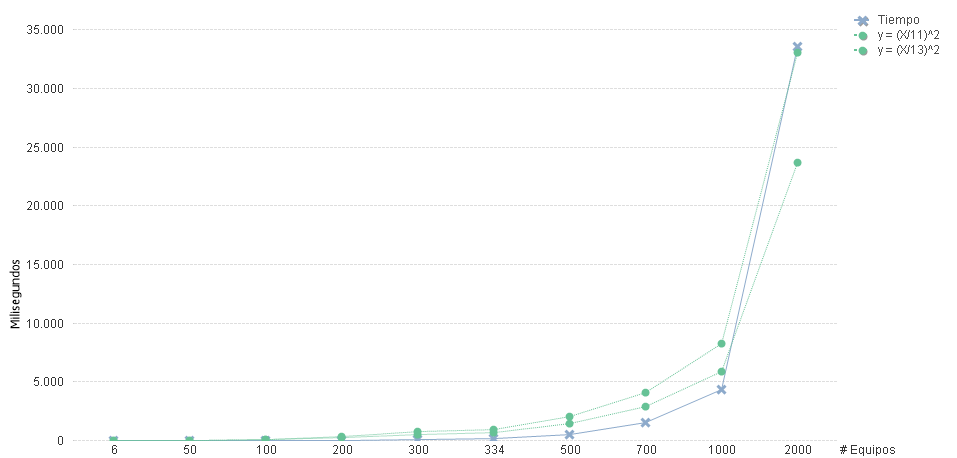
\includegraphics[width=1\textwidth]{IMG/gauss cuadrativo.png}
\caption{Gauss cuadratico}
\label{fig:Gauss cuadratico}
\end{figure}

\\

Luego observamos la misma gráfica pero con lineas de referencia de 2 funciones cubicas. \\

\begin{figure}[H]
\centering
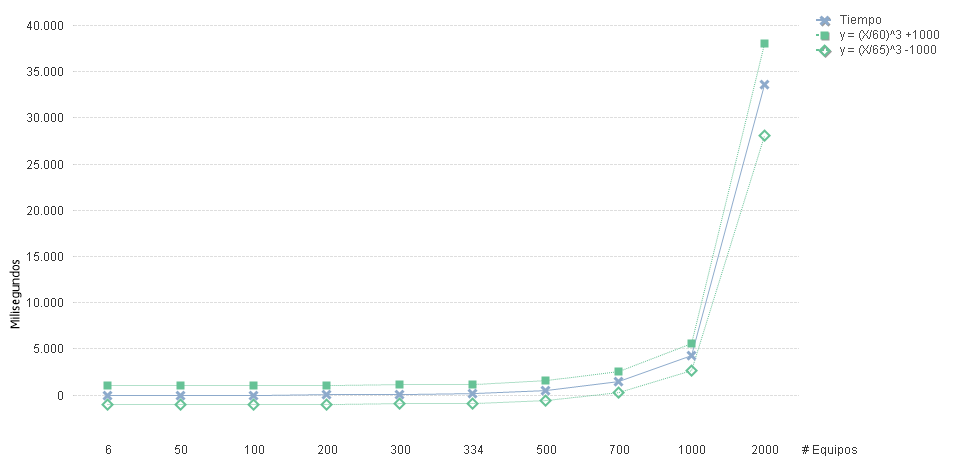
\includegraphics[width=1\textwidth]{IMG/gauss cubico.png}
\caption{Gauss cubico}
\label{fig:Gauss cubico}
\end{figure}

\\
Ejecutamos los test para nuestra implementacion de Cholesky.A continuación se muestran los resultados de tiempos de ejecucion dependiendo la cantidad de equipos.
Para mostrar la complejidad cúbica del algoritmo lo hemos encerrado entre 2 funciones cuadráticas que evidencian que no pueden contener la curva de tiempos de nuestro algoritmo.\\


\begin{figure}[H]
\centering
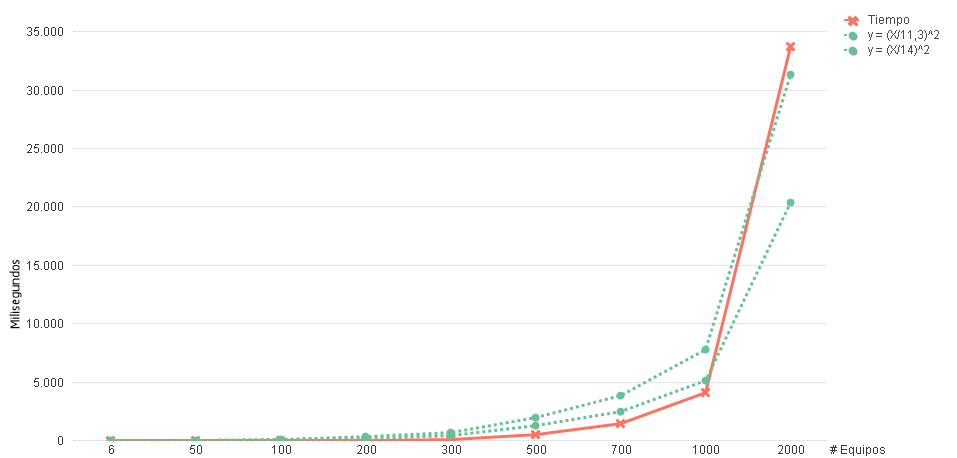
\includegraphics[width=1\textwidth]{IMG/cholesky cuadratico.png}
\caption{Cholesky cuadratico}
\label{fig:Cholesky cuadratico}
\end{figure}

\\

Luego observamos la misma grafica pero con lineas de referencia de 2 funciones cúbicas.\\

\begin{figure}[H]
\centering
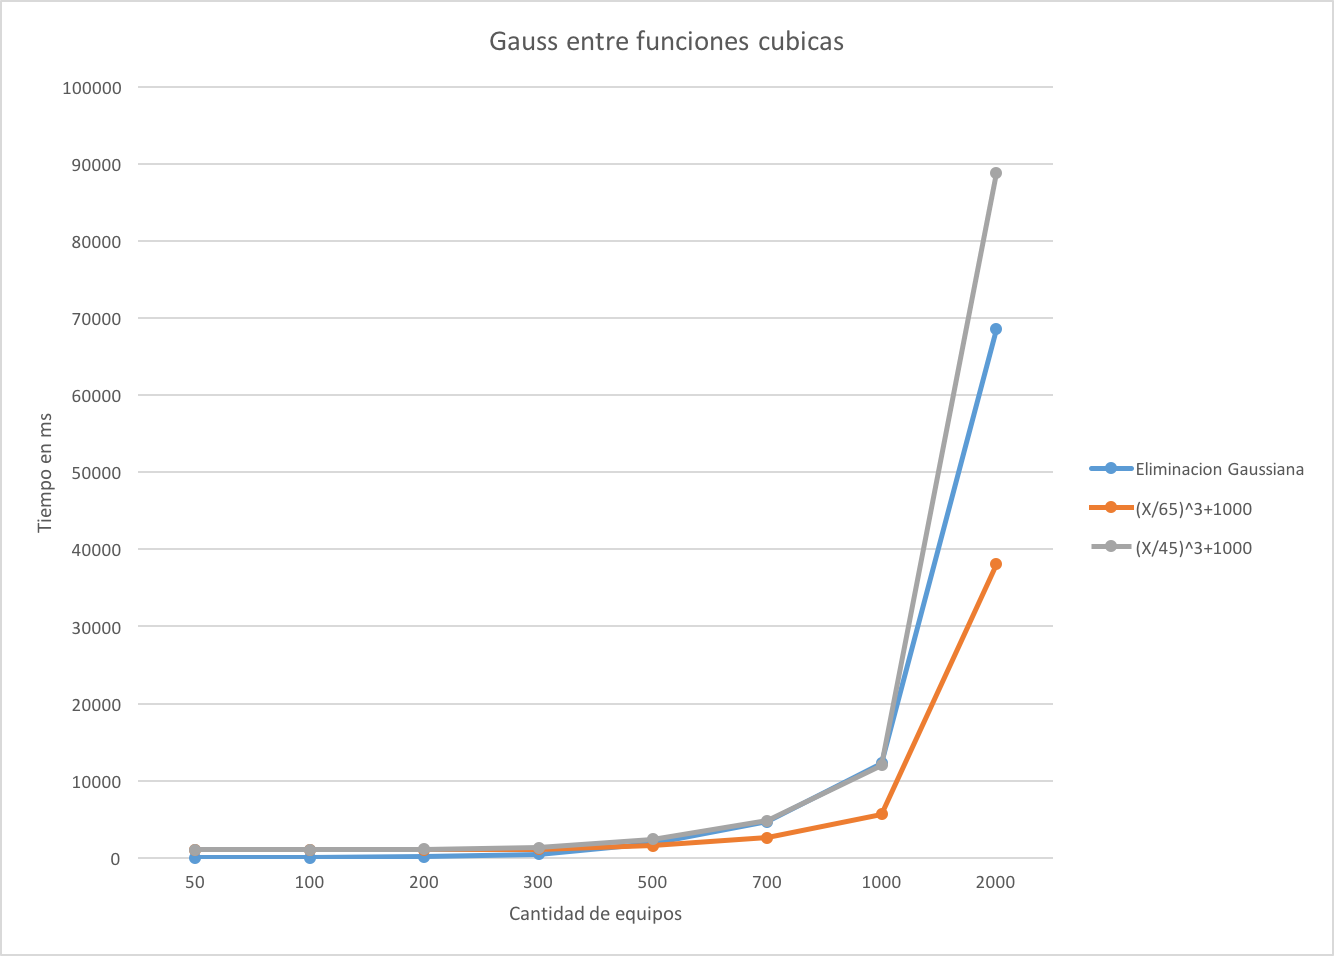
\includegraphics[width=1\textwidth]{IMG/gaussEntreCubicas.png}
\caption{Cholesky cubico}
\label{fig:Cholesky cubico}
\end{figure}

\\

Si comparamos ambos algoritmos, podemos comprobar que nuestra hipotesis de que cholesky demora menos tiempo es correcta, como se puede ver en la siguiente grafica.

\begin{figure}[H]
\centering
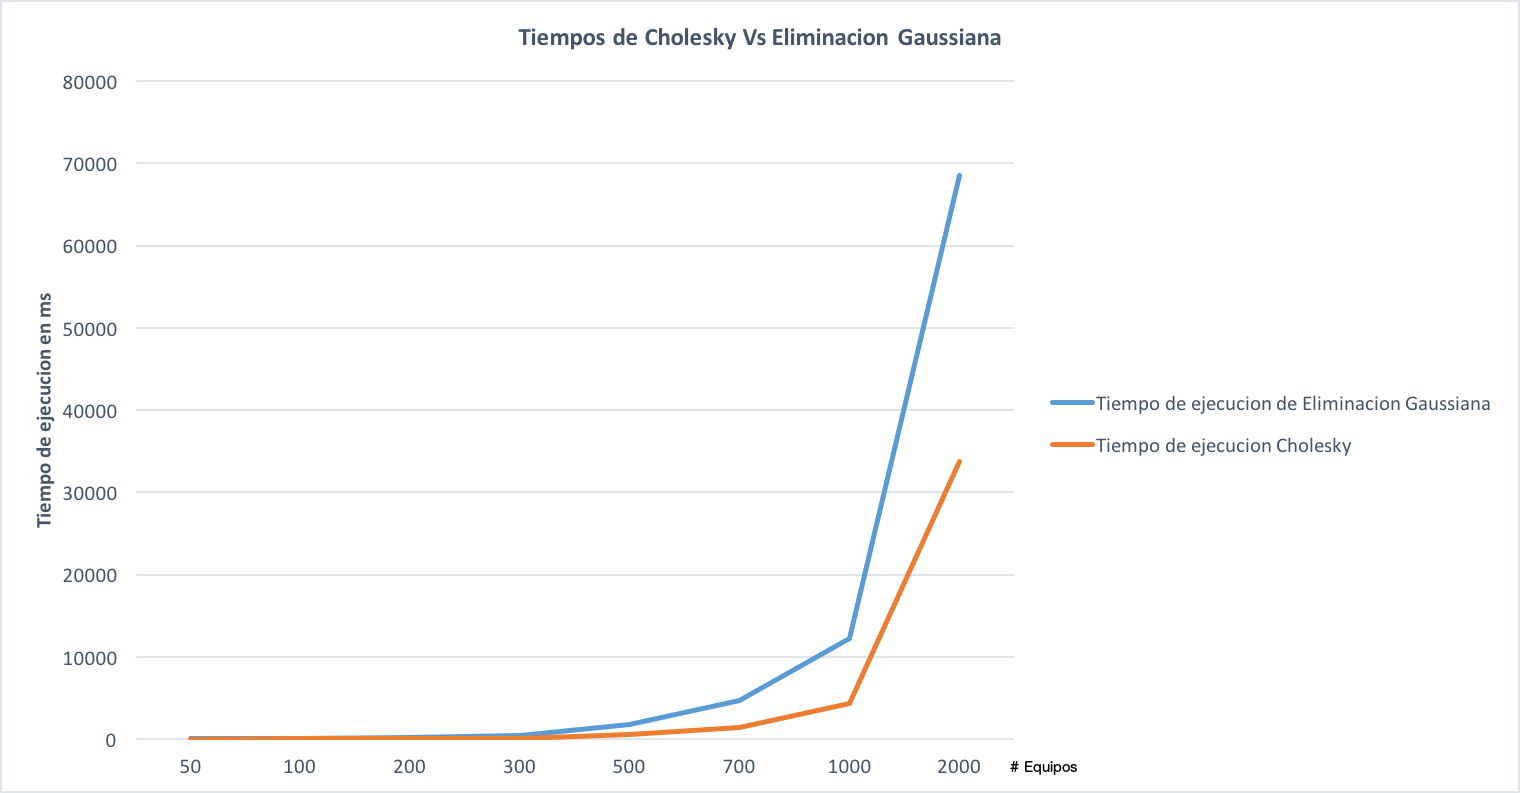
\includegraphics[width=1\textwidth]{IMG/tiemposgsvscholesky.png}
\end{figure}


Ejecutamos los test para nuestra implementacion de WP. A continuación se muestran los resultados de tiempos de ejecucion dependiendo la cantidad de equipos: \\


\begin{figure}[H]
\centering
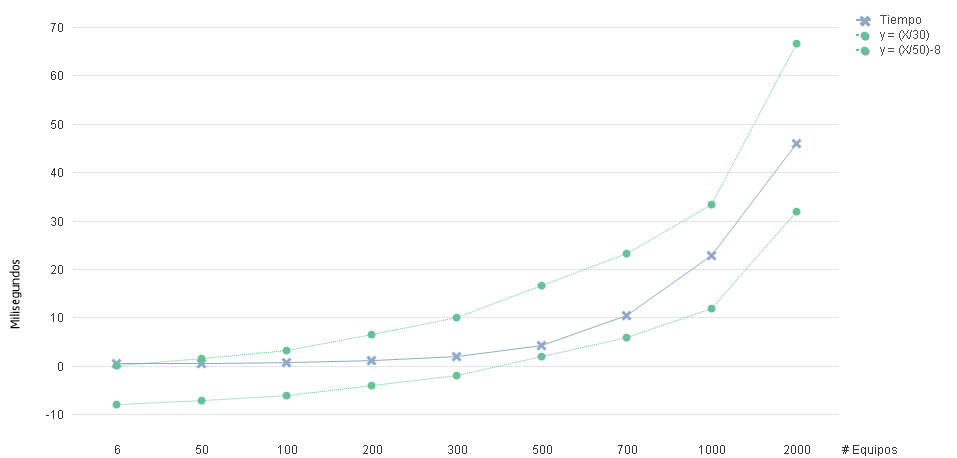
\includegraphics[width=1\textwidth]{IMG/wp lineal.png}
\caption{WP lineal}
\label{fig:WP lineal}
\end{figure}

\\


Cuando leimos el enunciado encontramos una frase que nos llamo la atención y era la siguiente: \\

\"Se pide comparar, para distintos tamaños de matrices, el tiempo de computo requerido para cada metodo en el contexto donde la información de la matriz del sistema (C) se mantiene invariante, 
pero varia el termino independiente (b)\"\\

Entendimos que nuestros tiempos de calculo no debian variar con la modificacion del termino independiente, pero para resolver esta incognita decidimos realizar la prueba.

Lo que hicimos fue tomar una matriz C, calcularle CMM, luego modificar algunos partidos de la matriz y cambiarlos (esto significa cambiar el resultado de ganados\/perdidos) y calculamos 
nuevamente CMM. \\

Nuestra experimentación intenta demostrar que el tiempo de cálculo no cambia, aunque se varie el termino independiente.
A continuación se grafican ambos tiempos.\\

\begin{figure}[H]
\centering
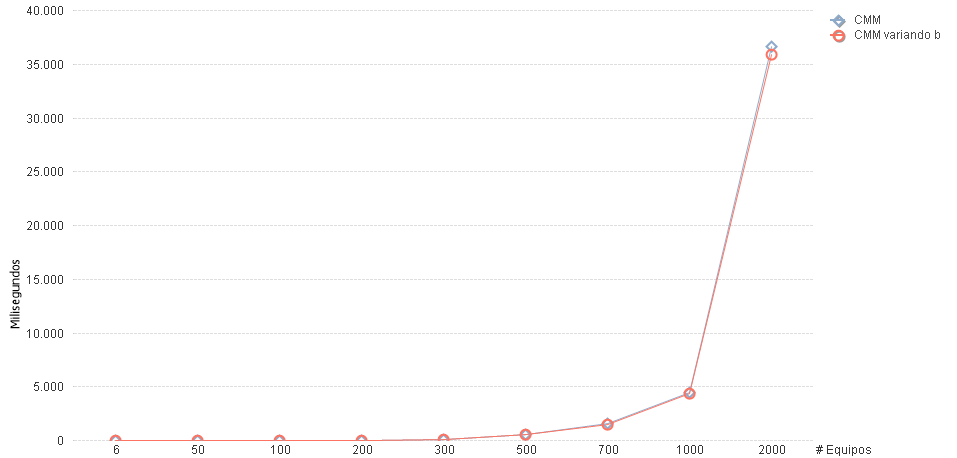
\includegraphics[width=1\textwidth]{IMG/Cholesky con otro termino independiente.png}
\caption{Cholesky con otro termino independiente}
\label{fig:Cholesky con otro termino independiente}
\end{figure}
